\chapter{Подход к вычислению КС-запросов к графам с использованием операций линейной алгебры}\label{ch:ch2}

Подход. Все рассматриваем на примере.

Соотношение шага вывода для грамматики и операции над матрицами. Все над матрицами с элементами --- множествами нетерминалов.

Переход к булевым полукольцам.


Сначала имеем матрицы с информацией о ребрах в графе (матрицы смежности). Потом, используя матричное умножение и другие операции для конкатенации путей в соответствии с шагом вывода грамматики. В результате будем иметь матрицы с информацией об искомых путях. По ним можно получить ответ на исходный КС-запрос.


	\begin{figure}
		\begin{center}
		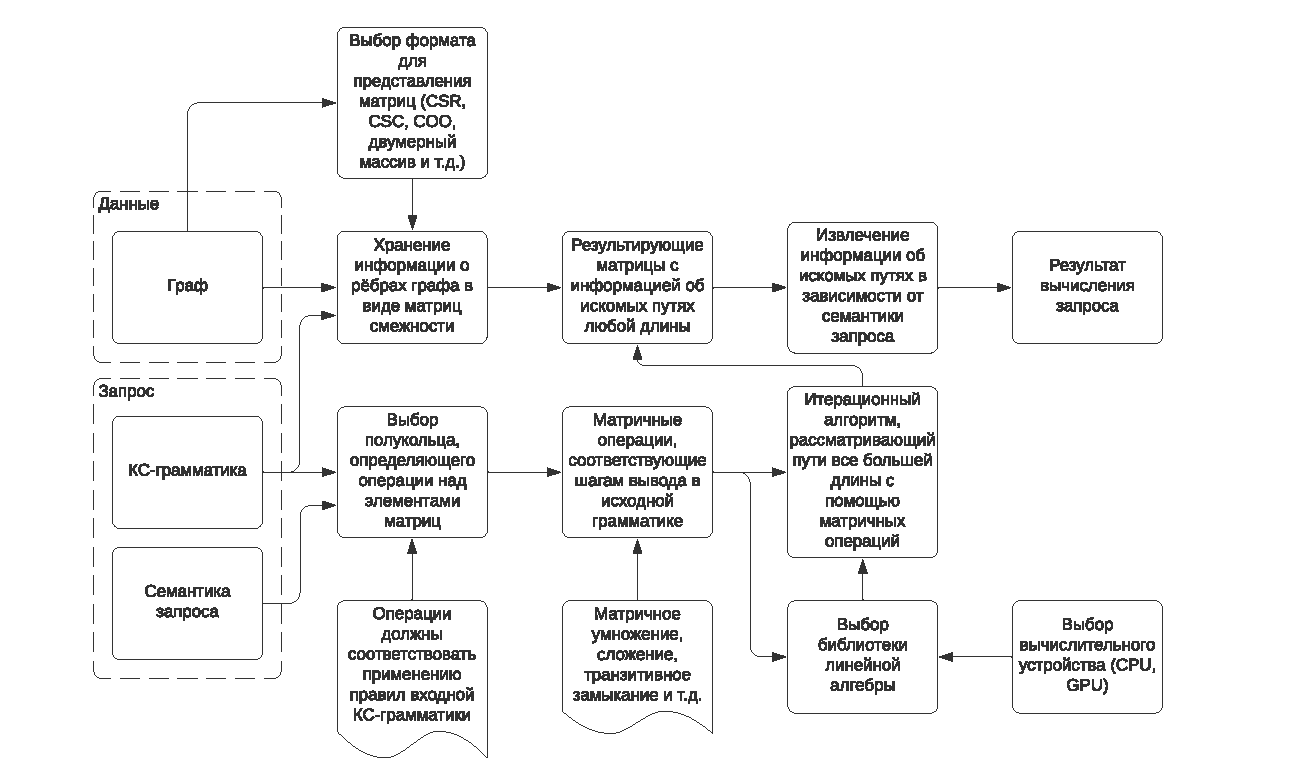
\includegraphics[height=12cm]{dissertation/images/schema.pdf}
	\end{center}
	\caption{Схема подхода к вычислению КС-запросов с помощью линейной алгебры.}
	\end{figure}

	


\FloatBarrier
